\begin{figure*}[t]
\centering\begin{tikzpicture}
\begin{groupplot}[group style={group size=3 by 2,horizontal sep=9mm,vertical sep=9mm},
 width=.27\textwidth,height=39mm,scale only axis=true,
 xmin=2016.8,xmax=2021.2,ymin=0,ymax=50,xtick={2017,2019,2021},xticklabels={17,19,21},ytick={0,20,40},
 tick label style={font=\scriptsize},title style={font=\small},ylabel style={font=\scriptsize},
 axis line style={gray},ymajorgrids=true,grid style={gray!18}]
\nextgroupplot[title={Romantic affection},ylabel={Recordings (\%)}]
\addplot[name path=lower0,draw=none] coordinates {(2017.000000,34.771657) (2018.000000,32.469527) (2019.000000,32.204276) (2020.000000,31.313403) (2021.000000,33.037893)};
\addplot[name path=upper0,draw=none] coordinates {(2017.000000,45.437784) (2018.000000,44.472891) (2019.000000,46.480589) (2020.000000,47.452949) (2021.000000,47.384528)};
\addplot[blue!13,draw=none] fill between[of=lower0 and upper0];
\addplot[blue,thick,mark=*,mark size=1.3pt] coordinates {(2017.000000,40.667626) (2018.000000,39.169534) (2019.000000,39.231390) (2020.000000,39.211221) (2021.000000,40.038148)};
\addplot[orange,thick,dashed,mark=square*,mark size=1.3pt] coordinates {(2017.000000,40.843806) (2018.000000,41.551724) (2019.000000,41.896272) (2020.000000,41.371994) (2021.000000,40.084986)};
\nextgroupplot[title={Sexual explicitness},ylabel={}]
\addplot[name path=lower1,draw=none] coordinates {(2017.000000,5.909948) (2018.000000,7.916010) (2019.000000,9.312452) (2020.000000,10.167596) (2021.000000,8.295344)};
\addplot[name path=upper1,draw=none] coordinates {(2017.000000,8.914187) (2018.000000,13.132479) (2019.000000,15.643946) (2020.000000,17.565024) (2021.000000,15.501254)};
\addplot[blue!13,draw=none] fill between[of=lower1 and upper1];
\addplot[blue,thick,mark=*,mark size=1.3pt] coordinates {(2017.000000,7.667900) (2018.000000,10.380642) (2019.000000,12.192882) (2020.000000,13.209204) (2021.000000,11.254716)};
\addplot[orange,thick,dashed,mark=square*,mark size=1.3pt] coordinates {(2017.000000,6.956912) (2018.000000,9.425287) (2019.000000,14.910859) (2020.000000,16.053748) (2021.000000,19.688385)};
\nextgroupplot[title={Materialism},ylabel={}]
\addplot[name path=lower2,draw=none] coordinates {(2017.000000,6.863643) (2018.000000,9.763686) (2019.000000,8.354031) (2020.000000,9.764218) (2021.000000,10.235561)};
\addplot[name path=upper2,draw=none] coordinates {(2017.000000,13.590013) (2018.000000,17.333145) (2019.000000,18.312764) (2020.000000,20.959022) (2021.000000,17.996222)};
\addplot[blue!13,draw=none] fill between[of=lower2 and upper2];
\addplot[blue,thick,mark=*,mark size=1.3pt] coordinates {(2017.000000,10.590463) (2018.000000,14.908394) (2019.000000,14.086727) (2020.000000,15.500047) (2021.000000,14.370067)};
\addplot[orange,thick,dashed,mark=square*,mark size=1.3pt] coordinates {(2017.000000,6.328546) (2018.000000,8.735632) (2019.000000,7.860616) (2020.000000,7.567185) (2021.000000,12.252125)};
\nextgroupplot[title={Crime},ylabel={Recordings (\%)}]
\addplot[name path=lower3,draw=none] coordinates {(2017.000000,3.751466) (2018.000000,4.795346) (2019.000000,4.711368) (2020.000000,4.533178) (2021.000000,5.213941)};
\addplot[name path=upper3,draw=none] coordinates {(2017.000000,8.122014) (2018.000000,10.944824) (2019.000000,11.878786) (2020.000000,15.202549) (2021.000000,14.404351)};
\addplot[blue!13,draw=none] fill between[of=lower3 and upper3];
\addplot[blue,thick,mark=*,mark size=1.3pt] coordinates {(2017.000000,6.696014) (2018.000000,8.678108) (2019.000000,9.234035) (2020.000000,10.810769) (2021.000000,10.406582)};
\addplot[orange,thick,dashed,mark=square*,mark size=1.3pt] coordinates {(2017.000000,4.443447) (2018.000000,4.712644) (2019.000000,5.105348) (2020.000000,4.596888) (2021.000000,6.161473)};
\nextgroupplot[title={Weapons},ylabel={}]
\addplot[name path=lower4,draw=none] coordinates {(2017.000000,1.989334) (2018.000000,3.036415) (2019.000000,3.045682) (2020.000000,3.684788) (2021.000000,3.565187)};
\addplot[name path=upper4,draw=none] coordinates {(2017.000000,5.030013) (2018.000000,7.771171) (2019.000000,8.074075) (2020.000000,11.641704) (2021.000000,10.062843)};
\addplot[blue!13,draw=none] fill between[of=lower4 and upper4];
\addplot[blue,thick,mark=*,mark size=1.3pt] coordinates {(2017.000000,3.849540) (2018.000000,5.817621) (2019.000000,6.129526) (2020.000000,7.851988) (2021.000000,7.383677)};
\addplot[orange,thick,dashed,mark=square*,mark size=1.3pt] coordinates {(2017.000000,2.827648) (2018.000000,2.816092) (2019.000000,3.403566) (2020.000000,3.677511) (2021.000000,4.249292)};
\nextgroupplot[title={Heartbreak},ylabel={}]
\addplot[name path=lower5,draw=none] coordinates {(2017.000000,19.287839) (2018.000000,18.413000) (2019.000000,17.997344) (2020.000000,17.984207) (2021.000000,20.012556)};
\addplot[name path=upper5,draw=none] coordinates {(2017.000000,24.584372) (2018.000000,25.113938) (2019.000000,27.742375) (2020.000000,28.169940) (2021.000000,30.729568)};
\addplot[blue!13,draw=none] fill between[of=lower5 and upper5];
\addplot[blue,thick,mark=*,mark size=1.3pt] coordinates {(2017.000000,22.184707) (2018.000000,21.807672) (2019.000000,23.141389) (2020.000000,23.056031) (2021.000000,25.105022)};
\addplot[orange,thick,dashed,mark=square*,mark size=1.3pt] coordinates {(2017.000000,21.409336) (2018.000000,23.390805) (2019.000000,25.283630) (2020.000000,26.732673) (2021.000000,31.090652)};
\end{groupplot}\end{tikzpicture}
\caption{International trajectories, 2017--2021. Blue circles: equal-market means for the same 55 markets in all five years; orange dashed squares: Brazil. Bands are the middle 50\% of market values, not confidence intervals. Each theme uses the same 0--50\% axis; substantial presence means intensity $\geq2$. Markets have at least 300 classified recordings and 50\% classification coverage in every year. The changing annual repertoires, not changes within a song, are measured.}
\label{fig:global-time}
\end{figure*}

\begin{figure}[t]
\centering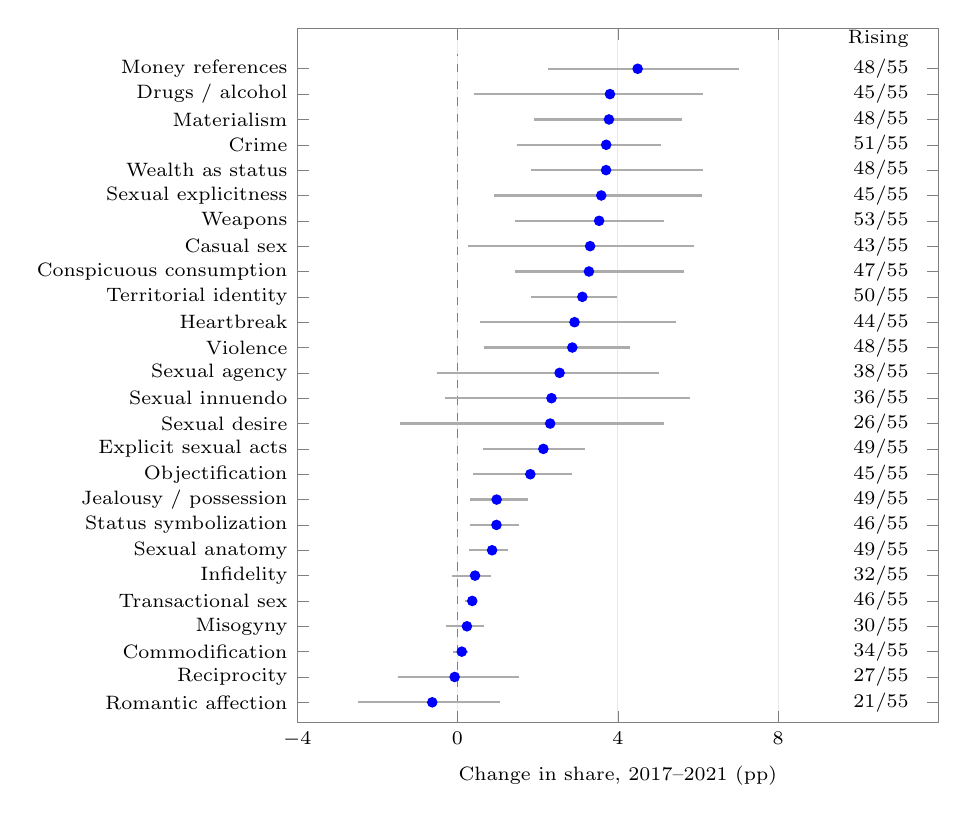
\begin{tikzpicture}
\begin{axis}[width=\dimexpr\columnwidth-24mm\relax,height=104mm,scale only axis=false,
 xmin=-4,xmax=12,ymin=.2,ymax=27.6,xtick={-4,0,4,8},ytick={26,25,24,23,22,21,20,19,18,17,16,15,14,13,12,11,10,9,8,7,6,5,4,3,2,1},yticklabels={{Money references},{Drugs / alcohol},{Materialism},{Crime},{Wealth as status},{Sexual explicitness},{Weapons},{Casual sex},{Conspicuous consumption},{Territorial identity},{Heartbreak},{Violence},{Sexual agency},{Sexual innuendo},{Sexual desire},{Explicit sexual acts},{Objectification},{Jealousy / possession},{Status symbolization},{Sexual anatomy},{Infidelity},{Transactional sex},{Misogyny},{Commodification},{Reciprocity},{Romantic affection}},
 xlabel={Change in share, 2017--2021 (pp)},xlabel style={font=\scriptsize},tick label style={font=\scriptsize},
 xmajorgrids=true,grid style={gray!18},axis line style={gray}]
\draw[gray,dashed] (axis cs:0,.3)--(axis cs:0,26.6);
\draw[gray!65,thick] (axis cs:2.267652,26)--(axis cs:7.022541,26);
\node[font=\scriptsize,anchor=east] at (axis cs:11.5,26) {48/55};
\draw[gray!65,thick] (axis cs:0.410851,25)--(axis cs:6.117446,25);
\node[font=\scriptsize,anchor=east] at (axis cs:11.5,25) {45/55};
\draw[gray!65,thick] (axis cs:1.901706,24)--(axis cs:5.611154,24);
\node[font=\scriptsize,anchor=east] at (axis cs:11.5,24) {48/55};
\draw[gray!65,thick] (axis cs:1.477499,23)--(axis cs:5.067675,23);
\node[font=\scriptsize,anchor=east] at (axis cs:11.5,23) {51/55};
\draw[gray!65,thick] (axis cs:1.839363,22)--(axis cs:6.126683,22);
\node[font=\scriptsize,anchor=east] at (axis cs:11.5,22) {48/55};
\draw[gray!65,thick] (axis cs:0.900828,21)--(axis cs:6.093631,21);
\node[font=\scriptsize,anchor=east] at (axis cs:11.5,21) {45/55};
\draw[gray!65,thick] (axis cs:1.440705,20)--(axis cs:5.143227,20);
\node[font=\scriptsize,anchor=east] at (axis cs:11.5,20) {53/55};
\draw[gray!65,thick] (axis cs:0.252737,19)--(axis cs:5.901170,19);
\node[font=\scriptsize,anchor=east] at (axis cs:11.5,19) {43/55};
\draw[gray!65,thick] (axis cs:1.428501,18)--(axis cs:5.661177,18);
\node[font=\scriptsize,anchor=east] at (axis cs:11.5,18) {47/55};
\draw[gray!65,thick] (axis cs:1.837014,17)--(axis cs:3.978834,17);
\node[font=\scriptsize,anchor=east] at (axis cs:11.5,17) {50/55};
\draw[gray!65,thick] (axis cs:0.574003,16)--(axis cs:5.449409,16);
\node[font=\scriptsize,anchor=east] at (axis cs:11.5,16) {44/55};
\draw[gray!65,thick] (axis cs:0.670765,15)--(axis cs:4.292003,15);
\node[font=\scriptsize,anchor=east] at (axis cs:11.5,15) {48/55};
\draw[gray!65,thick] (axis cs:-0.518891,14)--(axis cs:5.030915,14);
\node[font=\scriptsize,anchor=east] at (axis cs:11.5,14) {38/55};
\draw[gray!65,thick] (axis cs:-0.318277,13)--(axis cs:5.790287,13);
\node[font=\scriptsize,anchor=east] at (axis cs:11.5,13) {36/55};
\draw[gray!65,thick] (axis cs:-1.446731,12)--(axis cs:5.155236,12);
\node[font=\scriptsize,anchor=east] at (axis cs:11.5,12) {26/55};
\draw[gray!65,thick] (axis cs:0.638187,11)--(axis cs:3.174208,11);
\node[font=\scriptsize,anchor=east] at (axis cs:11.5,11) {49/55};
\draw[gray!65,thick] (axis cs:0.385005,10)--(axis cs:2.858504,10);
\node[font=\scriptsize,anchor=east] at (axis cs:11.5,10) {45/55};
\draw[gray!65,thick] (axis cs:0.321588,9)--(axis cs:1.761613,9);
\node[font=\scriptsize,anchor=east] at (axis cs:11.5,9) {49/55};
\draw[gray!65,thick] (axis cs:0.319422,8)--(axis cs:1.538841,8);
\node[font=\scriptsize,anchor=east] at (axis cs:11.5,8) {46/55};
\draw[gray!65,thick] (axis cs:0.296223,7)--(axis cs:1.264193,7);
\node[font=\scriptsize,anchor=east] at (axis cs:11.5,7) {49/55};
\draw[gray!65,thick] (axis cs:-0.129502,6)--(axis cs:0.841650,6);
\node[font=\scriptsize,anchor=east] at (axis cs:11.5,6) {32/55};
\draw[gray!65,thick] (axis cs:0.182799,5)--(axis cs:0.485998,5);
\node[font=\scriptsize,anchor=east] at (axis cs:11.5,5) {46/55};
\draw[gray!65,thick] (axis cs:-0.294200,4)--(axis cs:0.667159,4);
\node[font=\scriptsize,anchor=east] at (axis cs:11.5,4) {30/55};
\draw[gray!65,thick] (axis cs:-0.112472,3)--(axis cs:0.256888,3);
\node[font=\scriptsize,anchor=east] at (axis cs:11.5,3) {34/55};
\draw[gray!65,thick] (axis cs:-1.495781,2)--(axis cs:1.526836,2);
\node[font=\scriptsize,anchor=east] at (axis cs:11.5,2) {27/55};
\draw[gray!65,thick] (axis cs:-2.478436,1)--(axis cs:1.060692,1);
\node[font=\scriptsize,anchor=east] at (axis cs:11.5,1) {21/55};
\addplot[only marks,blue,mark=*,mark size=1.7pt] coordinates {(4.495539,26) (3.804479,25) (3.779604,24) (3.710568,23) (3.707348,22) (3.586817,21) (3.534137,20) (3.309420,19) (3.279988,18) (3.115725,17) (2.920314,16) (2.865182,15) (2.548219,14) (2.345754,13) (2.312660,12) (2.142570,11) (1.817757,10) (0.977507,9) (0.972531,8) (0.863537,7) (0.437759,6) (0.367759,5) (0.235336,4) (0.106954,3) (-0.070506,2) (-0.629478,1)};
\node[font=\scriptsize,anchor=east] at (axis cs:11.5,27.2) {Rising};
\end{axis}\end{tikzpicture}
\caption{Changes in all 26 dimensions in the fixed 55-market panel. Blue points: mean paired market change; gray segments: interquartile range of market changes. Right-hand counts show markets with a positive change. ``pp'' means percentage points. These spreads describe observed markets, not sampling confidence.}
\label{fig:global-changes}
\end{figure}

\begin{figure}[t]
\centering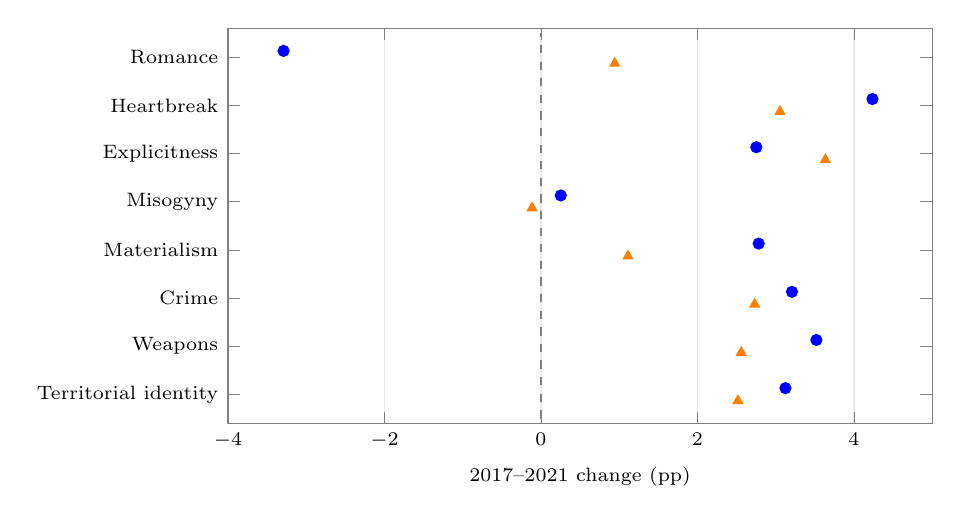
\begin{tikzpicture}
\begin{axis}[width=\dimexpr\columnwidth-16mm\relax,height=66mm,
 xmin=-4,xmax=5,ymin=.4,ymax=8.6,xtick={-4,-2,0,2,4},ytick={8,7,6,5,4,3,2,1},
 yticklabels={Romance,Heartbreak,Explicitness,Misogyny,Materialism,Crime,Weapons,Territorial identity},
 xlabel={2017--2021 change (pp)},xlabel style={font=\scriptsize},tick label style={font=\scriptsize},
 xmajorgrids=true,grid style={gray!18},axis line style={gray}]
\draw[gray,dashed] (axis cs:0,.5)--(axis cs:0,8.5);
\addplot[only marks,blue,mark=*,mark size=2pt] coordinates {(-3.289687,8.130) (4.237042,7.130) (2.752028,6.130) (0.253379,5.130) (2.782451,4.130) (3.207601,3.130) (3.519905,2.130) (3.124103,1.130)};
\addplot[only marks,orange,mark=triangle*,mark size=2pt] coordinates {(0.942803,7.870) (3.055312,6.870) (3.635211,5.870) (-0.113495,4.870) (1.112607,3.870) (2.731079,2.870) (2.560362,1.870) (2.517819,0.870)};
\end{axis}\end{tikzpicture}
\caption{Chart-family contrast in the same 52 markets. Blue circles: Top 200 (source union, IDs deduplicated); orange triangles: Viral 50. Each panel has at least 300 classified IDs and 50\% classification coverage in every full year. The romance trend changes direction across chart families; growth of status and conflict themes persists.}
\label{fig:family-trends}
\end{figure}

\begin{figure*}[t]
\centering\begin{tikzpicture}
\begin{groupplot}[group style={group size=3 by 2,horizontal sep=9mm,vertical sep=9mm},
 width=.265\textwidth,height=31mm,scale only axis=true,
 xmin=2016.8,xmax=2021.2,ymin=-.75,ymax=.75,xtick={2017,2019,2021},xticklabels={17,19,21},ytick={-.5,0,.5},
 tick label style={font=\scriptsize},title style={font=\scriptsize},ylabel style={font=\scriptsize},
 axis line style={gray},ymajorgrids=true,grid style={gray!18}]
\nextgroupplot[title={Romance / youth unemployment ($n=53$)},ylabel={$
ho$}]
\draw[gray,dashed] (axis cs:2016.8,0)--(axis cs:2021.2,0);
\addplot[teal,thick,mark=diamond*,mark size=1.5pt] coordinates {(2017.000000,-0.154975) (2018.000000,-0.078052) (2019.000000,-0.091761) (2020.000000,-0.040558) (2021.000000,-0.165215)};
\nextgroupplot[title={Materialism / PPP income ($n=54$)},ylabel={}]
\draw[gray,dashed] (axis cs:2016.8,0)--(axis cs:2021.2,0);
\addplot[teal,thick,mark=diamond*,mark size=1.5pt] coordinates {(2017.000000,0.430151) (2018.000000,0.411245) (2019.000000,0.607700) (2020.000000,0.590471) (2021.000000,0.534210)};
\nextgroupplot[title={Materialism / Gini ($n=39$)},ylabel={}]
\draw[gray,dashed] (axis cs:2016.8,0)--(axis cs:2021.2,0);
\addplot[teal,thick,mark=diamond*,mark size=1.5pt] coordinates {(2017.000000,-0.423972) (2018.000000,-0.301650) (2019.000000,-0.472131) (2020.000000,-0.504403) (2021.000000,-0.450000)};
\nextgroupplot[title={Misogyny / GII ($n=53$)},ylabel={$
ho$}]
\draw[gray,dashed] (axis cs:2016.8,0)--(axis cs:2021.2,0);
\addplot[teal,thick,mark=diamond*,mark size=1.5pt] coordinates {(2017.000000,-0.467534) (2018.000000,-0.462875) (2019.000000,-0.553284) (2020.000000,-0.551866) (2021.000000,-0.425067)};
\nextgroupplot[title={Violence / homicide ($n=47$)},ylabel={}]
\draw[gray,dashed] (axis cs:2016.8,0)--(axis cs:2021.2,0);
\addplot[teal,thick,mark=diamond*,mark size=1.5pt] coordinates {(2017.000000,-0.265264) (2018.000000,-0.333025) (2019.000000,-0.388645) (2020.000000,-0.385523) (2021.000000,-0.430054)};
\nextgroupplot[title={Territorial identity / urbanization ($n=54$)},ylabel={}]
\draw[gray,dashed] (axis cs:2016.8,0)--(axis cs:2021.2,0);
\addplot[teal,thick,mark=diamond*,mark size=1.5pt] coordinates {(2017.000000,0.238422) (2018.000000,0.234229) (2019.000000,0.360930) (2020.000000,0.316791) (2021.000000,0.289956)};
\end{groupplot}\end{tikzpicture}
\caption{Persistence of social associations, using a fixed market sample within each pair in every year. Points are separate-year Spearman correlations; $n$ counts markets, not people. World Bank data supply income, Gini, youth unemployment and urbanization; UNDP supplies GII; UNODC supplies homicide. No interpolation or pooled-year correlation is used. Stable directions describe aggregate associations and do not establish causes.}
\label{fig:social-time}
\end{figure*}